\newcommand{\cev}[1]{\reflectbox{\ensuremath{\vec{\reflectbox{\ensuremath{#1}}}}}}
\definecolor{in}{rgb}{0.89, 0.02, 0.17}
\definecolor{out}{rgb}{0.13, 0.55, 0.13}
\definecolor{highlight}{rgb}{0.47, 0.53, 0.6}

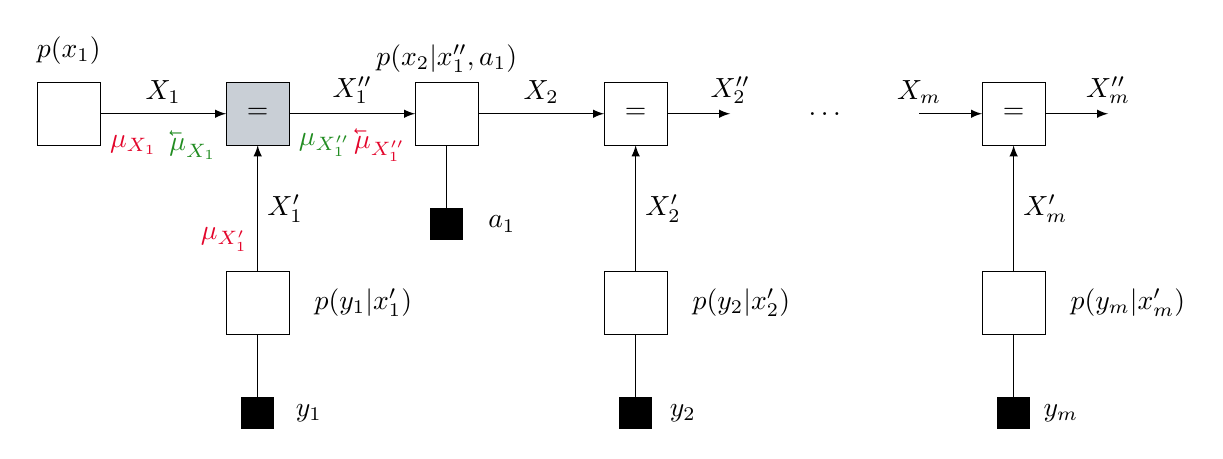
\begin{tikzpicture}

\draw  (-4.2,4.2) rectangle (-3.4,3.4);\node at (-3.8,4.6) {$p(x_1)$};
\draw [-latex](-3.4,3.8) -- (-1.8,3.8) node [midway, above, sloped]{$X_1$};, 
\draw  [color = black, fill = highlight, fill opacity=0.4, draw opacity = 1](-1.8,4.2) rectangle (-1,3.4) node [pos=0.5, color=black, opacity=1]{=};
\draw [-latex] (-1.4,1.8) -- (-1.4,3.4) node [midway, right]{$X'_1$};
\draw  (-1.8,1.8) rectangle (-1,1);\node at (-0.8,1.4) [anchor=west]{$p(y_1 | x'_1)$};
\draw (-1.4,0.2) -- (-1.4,1);
\draw  [fill=black](-1.6,0.2) rectangle (-1.2,-0.2);\node at (-0.75,0) {$y_1$};
\draw [-latex] (-1,3.8) -- (0.6,3.8) node [midway, above, sloped]{$X''_1$};
\node at (1.7,2.4) {$a_1$};
\draw [fill=black](0.8,2.6) rectangle (1.2,2.2);
\draw (1,2.6) -- (1,3.4);
\draw  (0.6,4.2) rectangle (1.4,3.4); \node at (1,4.5) {$p(x_2 | x''_1, a_1)$};
\draw [-latex](1.4,3.8) -- (3,3.8) node [midway, above, sloped]{$X_2$};
\draw  (3,4.2) rectangle (3.8,3.4) node [pos=0.5]{=};
\draw [-latex](3.4,1.8) -- (3.4,3.4) node [midway, right] {$X'_2$};
\draw  (3,1.8) rectangle (3.8,1); \node at (4,1.4) [anchor=west]{$p(y_2 | x'_2)$};
\draw (3.4,0.2) -- (3.4,1);
\draw  [fill=black](3.2,0.2) rectangle (3.6,-0.2); \node at (4,0) {$y_2$};
\draw [-latex](3.8,3.8) -- (4.6,3.8) node [above]{$X''_2$};

\node at (5.8,3.8) {$\dots$};
\draw [-latex](7,3.8) -- (7.8,3.8) node [pos=0, above]{$X_m$};
\draw  (7.8,4.2) rectangle (8.6,3.4) node [pos=0.5]{=};
\draw [-latex](8.2,1.8) -- (8.2,3.4) node [midway, right]{$X'_m$};
\draw  (7.8,1.8) rectangle (8.6,1);
\draw (8.2,0.2) -- (8.2,1);
\draw  [fill=black](8,0.2) rectangle (8.4,-0.2);\node at (8.8,0) {$y_m$};
\draw [-latex](8.6,3.8) -- (9.4,3.8) node [above]{$X''_m$};
\node [anchor=west] at (8.8,1.4) {$p(y_m | x'_m)$};


\node [anchor = west, color = in] at (-3.4,3.4) {$\Vec{\mu}_{X_1}$};
\node [anchor = east, color=out] at (-1.8,3.4) {$\cev{\mu}_{X_1}$};
\node [anchor=west, color=out] at (-1,3.4) {$\Vec{\mu}_{X''_1}$};
\node [anchor=east, color = in] at (-1.4,2.2) {$\Vec{\mu}_{X'_1}$};
\node [anchor = east, color = in] at (0.6,3.4) {$\cev{\mu}_{X''_1}$};
\end{tikzpicture}